Model in hand, we are finally ready to start tuning its hyperparameters on a dataset.
Where to start?
First, we processed the FER2013 dataset, with mean image substraction, and 1200 training set.
Then, we define the classification accuracy on the validation set as
the performance measure to be used to compare the performance of the different parameters on the validation set.

\begin{itemize}[topsep=-13pt]
\item \textbf{Select a reasonable network architecture}:\\
  After some hand-tuning of the hidden layer size, we decided to start with a single hidden layer of 512 hidden units.
  It seemed a reasonable tradeoff between complexity and training efficiency, and less likely to overfit.
  We set our model's momentum to 0.9 and its learning rate to a relatively small 1e-6
  since the magnitude of the gradient will be larger due to momentum.
  We set the batch size to a 100 and used 15 epochs.
  We added the following stopping criterion: stop if the error in the validation set does not decrease for three consecutive cycles.
  This will help increase our training efficiency.

\item \textbf{Optimize the learning rate}:\\
  Our experience hand-tuning the network as mentioned gave us a better idea of the range of learning rates we should test.
  We decided to initiate a grid search (of one parameter) for the learning rate in the range (1e-7, 1e-4).
  using the parameters found through hand-tuning in the previous section.
  Please find a below a graph showing the best validation accuracy for each learning rate tested in the range.
  \begin{figure}[!ht]
      \centering
      {{\includegraphics[scale = 0.50]{../src/optimizers/outputs/grid_search/learning_rate.png}}}
  \end{figure}

  The optimal learning rate was found at 6.5e-5.
  Please find below a plot of the training loss of our model, as well as its classification error on each set.
  \include*{../nets/optimal_learning_rate/info}

  \begin{figure}[!ht]
    \centering
        {{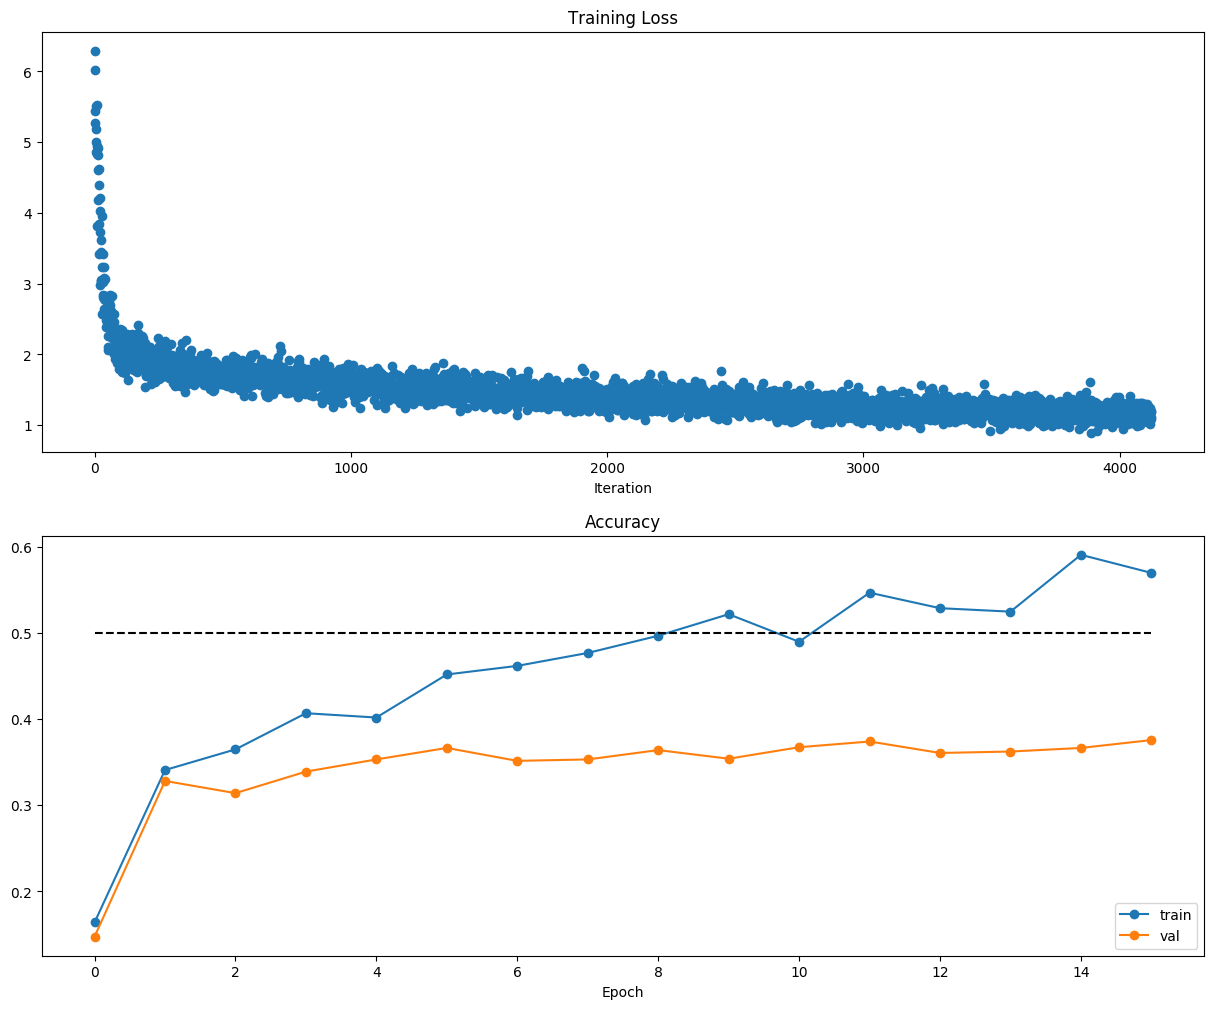
\includegraphics[scale = 0.32]{../nets/optimal_learning_rate/diagrams.png}}}  
  \end{figure}
  
\newpage  
\item \textbf{Using dropout}\\
  Now, keeping our optimal learning rate of 6.5e-5,
  we ran another grid search for dropout in the range (0.0, 1.0) to see if there was any improvement in the validation performance.
  Please find below a plot of the validation accuracy rate at each dropout rate examined.
  \begin{figure}[!ht]
    \centering
        {{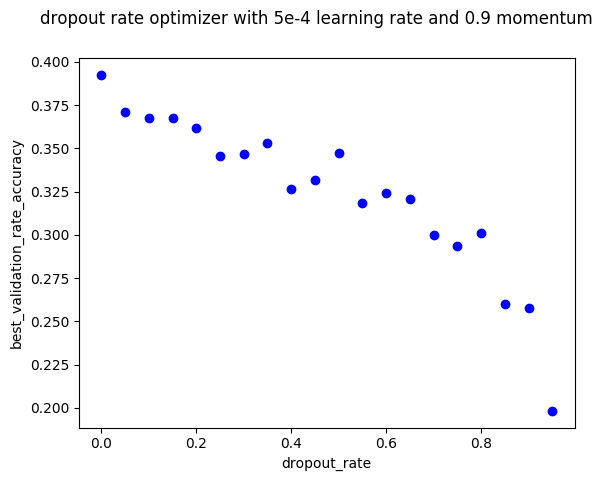
\includegraphics[scale = 0.50]{../src/optimizers/outputs/grid_search/dropout_rate.png}}}
  \end{figure}


\item \textbf{L2 vs dropout}:\\
  Let us now run a grid search to optimize L2 regularization,
  using the range (0.0, 1.0), to compare the performance against the dropout regularization.
  The highest validation accuracy rate obtained was 37.08\% with 0.85 L2 regularization constant.
  Please find below a plot of the validation accuracy rate at each L2 regularization rate tested.
  \begin{figure}[!ht]
    \centering
        {{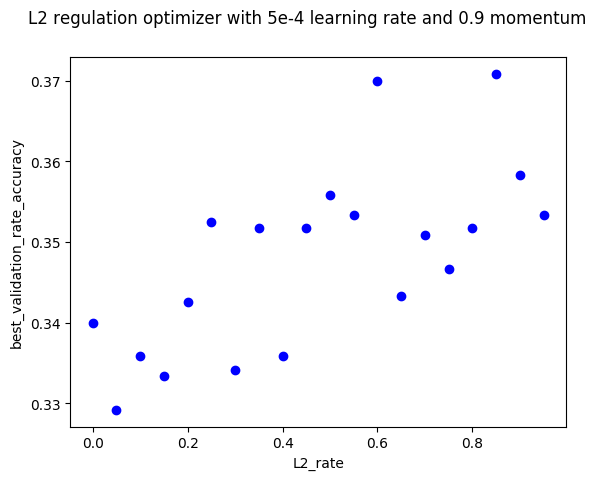
\includegraphics[scale = 0.50]{../src/optimizers/outputs/grid_search/L2_rate.png}}}
  \end{figure}

  
\item \textbf{Optimizing the topology of the layer}:\\
  Thus far, we have assumed that a neural net's hyperparameters are independent variables.
  Yet our experiences thus far have shown us that this is a false assumption.
  To optimize the topology of the layer, we have instead decided to run a random search,
  letting each hyperparameter be randomly drawn (within its respective range as defined in previous sections).
  This removes our false assumption of hyperparameters variable independence.
  We have found the optimal parameters to be:
  
\item \textbf{Performance metrics of network trained with the optimal set of parameters}:\\
  

  
\item \textbf{How to retrieve our best trained model}:\\
  You may retrieve and test our best trained model using our test.py file.
  Thank you.
\end{itemize}
  
